\chapter{概率论基础}\label{chap:prob}

本附录主要介绍Kolmogorov概率论,讨论只局限在数学层面,不涉及概率论的哲学讨论。

\section{从朴素概率论到公理化概率论}

\subsection{Kolmogorov概率论}
朴素的概率论通常讨论两种极端的情况,一个是可以用数数的方式来计算概率的情况,比如说掷骰子,另一个是用面积的方式来计算概率的情况,比如在随机选一个圆周上的点。这两个情况分别对应了\textbf{古典概型}和\textbf{几何概型}。

我们先给一些术语。考虑一个随机试验,它的所有可能结果组成的集合称为\textbf{样本空间}\index{样本空间},记为$\Omega$。样本空间的元素称为\textbf{样本点}\index{样本点},通常记为$\omega$. 样本空间的\emph{某些}子集被称为\textbf{事件}。我们来看看这些概念在朴素的概率论中都具体是什么。

\begin{example}[古典概型]
考虑先后掷两个骰子的情况。样本空间为
\[
    \Omega = \{ (i, j): 1 \leq i, j \leq 6 \}.
\]
样本点为$(i, j)$,表示第一个骰子掷出$i$点,第二个骰子掷出$j$点。“第一个骰子掷出$i$点”这个事件可以表示为$A_i = \{ (i, j): 1 \leq j \leq 6 \}$. “第一个骰子掷出$i$点,第二个骰子掷出$j$点”这个事件可以表示为$B_{ij} = \{ (i, j) \}$.
\end{example}

\begin{example}[几何概型]
考虑随机选一个圆周上的点的情况。如果用弧度来表示圆周上的点,那么样本空间为
\[
    \Omega = [0, 2\pi).
\]
样本点为$\omega$,表示选出点的弧度。事件$A = [0, \pi)$表示选出了上半圆周,事件$B = [0, \pi/2)\cup[\pi, 3\pi/2)$表示选出了右上或左下的$1/4$圆周。
\end{example}

那么,如何定义概率呢?朴素地说,概率是某个事件出现的可能性占总可能的比例。

对于古典概型,我们简单认为每个样本点出现的概率都是相同的,也就是说,如果用$p_\omega$表示样本点$\omega$出现的概率,那么对任意$\omega\in\Omega$,都有$p_\omega = 1/|\Omega|$. 于是,对于任意事件$A$,它发生的概率为
\[
    \sum_{\omega\in A} p_\omega = \frac{|A|}{|\Omega|}.
\]
例如在上面掷骰子的例子中,$p_\omega=1/36$,$A$发生的概率为$1/6$,$B$发生的概率为$1/36$.

对于几何概型,不能再用古典概型的方式定义概率。一段长为$2\pi$的圆弧上,一个点的长度当然是$0$,所以选到一个点的概率是$0$。计算选到上半圆周的概率,就是把所有上半圆周上的点的概率加起来,任意多个$0$相加依然还是$0$,所以这样的定义出来的概率永远是零,这样是不可行的。

朴素的直觉告诉我们,选到上半圆周的概率是$1/2$,因为上半圆周刚好占了半个圆周。所以几何概型的概率定义利用了\emph{体积}的概念。事件$A$的概率定义为
\[
    \frac{\text{事件$A$对应的体积}}{\text{样本空间$\Omega$对应的体积}}.
\]
这里体积应该按照广义上来理解,一维集合的体积就是长度,二维集合的体积就是面积,三维集合的体积就是体积,以此类推。例如在上面圆周的例子中,$A$对应的体积(长度)为$\pi$,$\Omega$对应的体积(长度)为$2\pi$,所以$A$发生的概率为$1/2$. 同理,$B$的概率也是$1/2$.

几何概型的定义非常微妙,因为我们并不知道如何定义“体积”。我们来看一个有趣的例子。

\begin{example}[Bertrand悖论]
考虑一个圆,它的半径为$1$. 现在我们随机地在圆上取一个弦,那么这个弦的长度超过$\sqrt{3}$(即圆内接正三角形的边长)的概率是多少?我们给出三种答案。
\begin{enumerate}[label=\textbf{解答\arabic*.},fullwidth,itemindent=2em]
    \item 不妨固定弦的其中一个点$A$,那么另一个点$B$可以在圆上等可能取。以$A$为顶点作圆内接正三角形$ACD$,弦的长度超过$\sqrt{3}$等价于$B$在弧$CD$上,所以概率为$1/3$.
    \item 弦长只与它到圆心的距离有关系,与方向无关。弦长超过$\sqrt{3}$等价于它到圆心的距离小于$1/2$,所以概率为$1/2$.
    \item 弦被它的中点唯一确定,弦长大于$\sqrt{3}$等价于中点落在一个半径为$1/2$的同心小圆内,所以概率为同心小圆面积比上大圆面积,即$(1/2)^2=1/4$.
\end{enumerate}
三种解答的示意图见下(从左到右分别是解答1到3):
\begin{center}
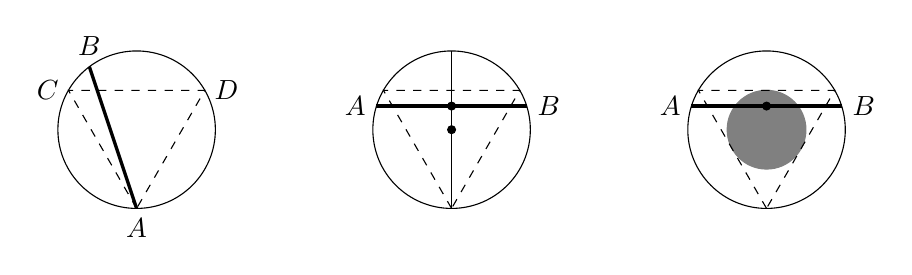
\begin{tikzpicture}
\draw (0,0) circle [radius=1];
\draw[dashed] (0,-1) node[below] {$A$} -- ({-sqrt(3)/2},0.5) node[left] {$C$} -- ({sqrt(3)/2},0.5) node[right] {$D$} -- cycle;
\draw[very thick] (0,-1) -- (-0.6,0.8) node[above] {$B$};

\draw (4,0) circle [radius=1];
\draw (4,-1) -- (4,1);
\draw[dashed] (4,-1)-- ({4-sqrt(3)/2},0.5)  -- ({4+sqrt(3)/2},0.5) -- cycle;
\draw[fill] (4,0) circle [radius=0.05];
\draw[fill] (4,0.3) circle [radius=0.05];
\draw[very thick] ({4-sqrt(1-0.3^2)},0.3) node[left] {$A$} -- ({4+sqrt(1-0.3^2)},0.3) node[right] {$B$};

\draw (8,0) circle [radius=1];
\draw[fill,gray] (8,0) circle [radius=0.5];
\draw[dashed] (8,-1)-- ({8-sqrt(3)/2},0.5)  -- ({8+sqrt(3)/2},0.5) -- cycle;
\draw[fill] (8,0.3) circle [radius=0.05];
\draw[very thick] ({8-sqrt(1-0.3^2)},0.3) node[left] {$A$} -- ({8+sqrt(1-0.3^2)},0.3) node[right] {$B$};
\end{tikzpicture}
\end{center}
\end{example}

因此,我们需要一个更加严格的定义来描述概率。首先注意到,概率应该是一个函数,它的值域是$[0,1]$. 那么,它的定义域应该是什么呢?我们已经看到,概率应该定义在\emph{事件}上,而非\emph{样本点}上。那么,概率可以定义在\emph{任意}事件上吗?这个问题的答案非常微妙,我们不在这里讨论。这里只是指出,我们关心的并不总是任意事件,而是一类被$\sigma$-代数所刻画的事件。

\begin{definition}[$\sigma$-代数]\index{$\sigma$-代数}
设$\Omega$是一个集合,$\mathscr{F}$是$\Omega$的子集的集合。如果$\mathscr{F}$满足
\begin{enumerate}
    \item $\Omega\in\mathscr{F}$;
    \item 如果$A\in\mathscr{F}$,则$A$的补集$\Omega\setminus A\in\mathscr{F}$;
    \item 如果$A_1,A_2,\ldots\in\mathscr{F}$,则$\bigcup_{i=1}^\infty A_i\in\mathscr{F}$.
\end{enumerate}
则称$\mathscr{F}$是$\Omega$上的一个 \textbf{$\sigma$-代数}。
\end{definition}

在样本空间中,我们要求事件也形成一个$\sigma$-代数。这样的$\sigma$-代数称为\textbf{事件域}\index{事件域},记为$\mathscr{F}$,关于这一定义的哲学讨论,可以见\Cref{chap:plausible-reasoning}. 接下来,我们给出Kolmogorov概率论的公理化定义。

\begin{definition}[概率空间,概率测度]\index{概率空间}\index{概率}\index{概率测度}
设$\Omega$是一个集合,$\mathscr{F}$是$\Omega$上的一个$\sigma$-代数。如果函数$\Pr:\mathscr{F}\to[0,1]$满足
\begin{enumerate}
    \item 正则性:$\Pr(\Omega)=1$;
    \item 可列可加性:如果$A_1,A_2,\dots\in\mathscr{F}$是两两不相交的事件,则
    \[
        \Pr\left(\bigcup_{i=1}^\infty A_i\right) = \sum_{i=1}^\infty \Pr(A_i),
    \]
    则称$(\Omega,\mathscr{F},\Pr)$是一个\textbf{概率空间},$\Pr$称为\textbf{概率测度}或\textbf{概率}。
\end{enumerate}
\end{definition}
容易证明,概率有如下性质:
\begin{proposition}
设$(\Omega,\mathscr{F},\Pr)$是一个概率空间,则:
\begin{enumerate}
    \item $\Pr(\varnothing)=0$;
    \item 单调性:对任意的$A,B\in\mathscr{F}$,如果$A\subseteq B$,则$\Pr(A)\leq\Pr(B)$;
    \item 有限可加性:对两两不相交的$A_1,A_2,\dots,A_n\in\mathscr{F}$,有
    \[
        \Pr\left(\bigcup_{i=1}^n A_i\right) = \sum_{i=1}^n \Pr(A_i).
    \]
\end{enumerate}
\end{proposition}
他们的证明都不困难,我们略去。

对于古典概型来说,我们容易写出它的概率空间。此时事件域恰好为所有$\Omega$的子集的集合,概率测度的定义也就是我们之前的定义。对于几何概型来说,这一定义需要克服很多技术层面的困难,我们不在这里讨论。

\subsection{条件概率,独立性}
接下来,我们讨论条件概率与独立性。我们还是看先后掷两个骰子的例子。如果掷完第一个骰子,我们马上观察结果,然后再掷第二个骰子,问第一个骰子是$i$,第二个是$j$的概率是多少?如果继续套用原来的概率空间,我们很快就会觉得不对劲。此时,第一个骰子完全没有随机性!所以朴素的直觉告诉我们,这里的概率应该有另一个依赖于第一次投骰子结果的定义,这样的概率就是\emph{条件概率}。

我们直接给出一般情况下条件概率的定义。

\begin{definition}[条件概率]\index{条件概率}
设$(\Omega,\mathscr{F},\Pr)$是一个概率空间,$A,B\in\mathscr{F}$是两个事件,且$\Pr(A)>0$. 则称
\[
    \Pr(B|A) = \frac{\Pr(A\cap B)}{\Pr(A)}
\]
是事件$B$在事件$A$发生的条件下发生的\textbf{条件概率}。
\end{definition}

以上定义要求$A$发生概率为正,然而$A$是零概率的时候也是可能有条件概率的。例如,
从$[0,1]\times[0,1]$中均匀地随机选一个点$(X,Y)$,观察它的横坐标$X$,不管什么样的$x$,$X=x$的概率都是$0$。然而,从朴素的直觉来看,条件在$X=x$上,$Y>1/2$的概率不仅存在,而且应该是$1/2$。在\Cref{sec:random-variable} 中,我们会针对一类特殊的事件,给出此时条件概率的定义。

我们继续看投两个骰子的例子。假设事件$A$是“第一个骰子是$i$“,事件$B$是“第二个骰子是$j$”。我们可以计算出$\Pr(B|A)=\Pr(B)=\frac{1}{6}$. 如果单看数学计算,这是一个非常神奇的式子:条件在$A$上和不条件在$A$上概率是一样的!从朴素的直觉来说,这件事情却并不神秘,因为第一个骰子的结果和第二个骰子的结果是不应该有关系的。我们把这种现象称为\textbf{独立性}。更一般地,对任意事件$A,B$,如果$\Pr(A)>0$,那么
\[\Pr(B|A)=\Pr(B)\iff \frac{\Pr(A\cap B)}{\Pr(A)}=\Pr(B)\iff \Pr(A\cap B)=\Pr(A)\Pr(B).\]
最后一个式子并不要求$\Pr(A)>0$,因此我们用它作为独立性的定义,这样定义可以不依赖条件概率。

\begin{definition}[独立性]\index{独立性}
设$(\Omega,\mathscr{F},\Pr)$是一个概率空间,$A,B\in\mathscr{F}$是两个事件。如果$\Pr(A\cap B)=\Pr(A)\Pr(B)$,则称事件$A$和$B$\textbf{相互独立}。

一般地,给定一个事件族$\mathscr{A}\subseteq\mathscr{F}$,如果对任意的有限个不同的$A_1,A_2,\ldots,A_n\in\mathscr{A}$,都有
\[
    \Pr\left(\bigcap_{i=1}^n A_i\right) = \prod_{i=1}^n \Pr(A_i),
\]
则称事件族$\mathscr{A}$中的事件是\textbf{相互独立}的。
\end{definition}

我们在定义中还给出了多个事件相互独立的定义,这一定义是说不管挑出其中多少个事件,他们都应该满足交的概率等于概率的积。这并不等价于任意两个事件都相互独立,我们看下面的例子。

\begin{example}
两个人进行石头剪刀布游戏,每个人独立等概率地出剪刀石头布. 考虑下面三个事件:$A=\{\text{甲出了石头}\}$,$B=\{\text{乙出了剪刀}\}$,$C=\{\text{甲赢}\}$.

容易算出,$\Pr(A\cap B)=\Pr(A)\Pr(B)=1/9$,$\Pr(A\cap C)=\Pr(A)\Pr(C)=1/9$,$\Pr(B\cap C)=\Pr(B)\Pr(C)=1/9$,所以$A,B,C$两两独立. 但是$A,B,C$不是相互独立的:$\Pr(A\cap B\cap C)=1/9\neq 1/27=\Pr(A)\Pr(B)\Pr(C)$.
\end{example}

这个例子说明,三个事件的独立性远比他们任意两个之间的独立性要复杂,三个事件可能放在一起才会出现不独立的情况。对于一般情况,这样的现象更加普遍,所以我们多个事件的独立性定义是要求任意有限个事件都独立,而不是任意两个事件都独立。

最后,我们给出条件概率的一些性质。

\begin{proposition}\label{prop:conditional-probability}
设$(\Omega,\mathscr{F},\Pr)$是一个概率空间,那么
\begin{enumerate}
    \item 对任意$A\in\mathscr{F}$满足$\Pr(A)>0$,$\Pr(\cdot|A)$也是一个概率测度;
    \item $\Pr(|\Omega)=\Pr(\cdot)$,
    \item 对任意$A\in\mathscr{F}$满足$\Pr(A)>0$,$\Pr(A|A)=1$.
\end{enumerate}
\end{proposition}
以上性质的证明都很简单,我们就不给出了。

\begin{theorem}[全概率公式]\index{全概率公式}\label{thm:total-probability}
设$(\Omega,\mathscr{F},\Pr)$是一个概率空间,$A_1,A_2,\ldots\in\mathscr{F}$是一列两两不相交的事件,且$\Pr(A_i)>0$,$\bigcup_{i=1}^\infty A_i=B$,则对任意的$C\in\mathscr{F}$,有
\[
    \Pr(C|B) = \sum_{i=1}^\infty \Pr(C|A_i)\Pr(A_i).
\]
特别地,对于有限个$A_i$,这一定理也成立。
\end{theorem}
\begin{proof}
注意到
\[
    \Pr(C) = \Pr(C\cap B) = \Pr\left(C\cap\bigcup_{i=1}^\infty A_i\right) = \Pr\left(\bigcup_{i=1}^\infty (C\cap A_i)\right) = \sum_{i=1}^\infty \Pr(C\cap A_i).
\]
最后一个等号是因为$C\cap A_i$两两不相交。另一方面,
\[
    \Pr(C\cap A_i) = \Pr(C|A_i)\Pr(A_i),
\]
所以
\[
    \Pr(C) = \sum_{i=1}^\infty \Pr(C|A_i)\Pr(A_i).
\]
对于有限个$A_i$,只需要把无穷求和改成有限求和,利用有限可加性即可即可。
\end{proof}

全概率公式是一种分而治之的思想,它把一个复杂的事件分解成若干个简单的事件,然后再把简单的事件的概率加起来。我们来看一个例子。

\begin{example}
    从装有$w$个白球和$b$个黑球的盒子中随机地取出一个球,不放回,再取出一个球。问第二个球是白球的概率是多少?

    设事件$A$是“第一个球是白球”,事件$B$是“第二个球是白球”。我们有
\begin{align*}
    \Pr(B) &= \Pr(B|A)\Pr(A) + \Pr(B|\bar{A})\Pr(\bar{A}) \\
    &=\frac{w-1}{w+b-1}\cdot\frac{w}{w+b} + \frac{w}{w+b-1}\cdot\frac{b}{w+b}\\
    &=\frac{w}{w+b}.
\end{align*}
    这里$\bar A$指的是$A$的补集,即“第一个球是黑球”。
\end{example}

\begin{theorem}[贝叶斯公式]\index{贝叶斯公式}\label{thm:bayes}
设$(\Omega,\mathscr{F},\Pr)$是一个概率空间,$A,B\in\mathscr{F}$且$\Pr(A),\Pr(B)>0$,则
\[
    \Pr(A|B) = \frac{\Pr(B|A)\Pr(A)}{\Pr(B)}.
\]
\end{theorem}
这一公式的证明几乎是显然的,我们略去。

一个特别重要的推论被称为\emph{链式法则}\index{链式法则},它是\emph{Bayes网络}\index{Bayes网络}的基础。

\begin{corollary}[链式法则]\index{链式法则}\label{cor:chain-rule}
设$(\Omega,\mathscr{F},\Pr)$是一个概率空间,$A_1,A_2,\ldots,A_n\in\mathscr{F}$,且$\Pr(A_1\cap A_2\cap\cdots\cap A_n)>0$,则
\begin{align*}
    &\Pr(A_1\cap A_2\cap\cdots\cap A_n)\\
    = &\Pr(A_1)\Pr(A_2|A_1)\Pr(A_3|A_1\cap A_2)\cdots\Pr(A_n|A_1\cap A_2\cap\cdots\cap A_{n-1}).
\end{align*}
\end{corollary}

我们也看一个例子。

\begin{example}[P\'olya的罐子]
    一个罐子装有$w$个白球和$b$个黑球,随机取出一个,观察它的颜色,放回,再放回相同颜色的$c$个球,再随机取一次,重复上述操作,如此反复$n$次,问每一次都取到白球的概率是多少?

    设事件$A_i$是“第$i$次取出的球是白球”。我们有
\begin{align*}
    \Pr(A_1)&=\frac{w}{w+b},\\
    \Pr(A_2|A_1)&=\frac{w+c}{w+b+c},\\
    \Pr(A_3|A_1\cap A_2)&=\frac{w+2c}{w+b+2c},\\
    &\cdots\\
    \Pr(A_n|A_1\cap A_2\cap\cdots\cap A_{n-1})&=\frac{w+nc}{w+b+nc}.
\end{align*}
    所以
\[
    \Pr(A_1\cap A_2\cap\cdots\cap A_n) = \frac{w}{w+b}\cdot\frac{w+c}{w+b+c}\cdots\frac{w+nc}{w+b+nc}.
\]
\end{example}

\begin{remark}
    在概率论中,我们经常要讨论事件的交,所以我们通常会把$A\cap B$简记为$AB$。此外,事件不相交我们也称之为\textbf{互斥}。事件$A$的补事件,即$\Omega\setminus A$.我们会记为$\bar{A}$或$A^c$.
    
    另外,我们也经常要讨论一个关于$\omega$的陈述$Q(\omega)$定义的事件$\{\omega\in\Omega:Q(\omega)\}$,在P\'olya的罐子的例子中,事件$A_1$其实就是由陈述$Q(\omega)$:“$\omega$中第一次取出的球是白球”定义的事件。在这种情况下,我们将这一事件简记为$\{Q\}$,它的概率就是$\Pr(\{Q\})$或者简记为$\Pr(Q)$。此时,事件交的概率也经常以逗号的形式写出,例如,$\Pr(A_1A_2)$我们会记为$\Pr(\text{第一次取出的球是白球},\text{第二次取出的球是白球})$. 这样的记号更直观,并且在随机变量部分会经常使用。
\end{remark}
\section{随机变量,分布函数}\label{sec:random-variable}

\section{随机变量的数字特征,期望}

\section{多元正态分布(Gauss向量)}